\documentclass[12pt]{article}

\usepackage{sbc-template}
\usepackage{graphicx,url}
\usepackage[utf8]{inputenc}
\usepackage[brazil]{babel}
\usepackage{booktabs}

     
\sloppy

\title{Análise Preditiva da Receita de Jogos na Plataforma Steam}

\author{Gabriel de França Marques (RA: 10395270)\inst{1}, Henrique Magno dos Santos(RA: 10335286)\inst{1}, \\ 
Pedro Machado Gomes Caixeta (RA: 10314309)\inst{1}}

\address{Ciência da Computação (CC) -- Faculdade de Ciência e Informação (FCI) -- \\
  Universidade Presbiteriana Mackenzie (UPM)
  \email{10395270@, 10335286@,
  10314309@mackenzista.com.br}
}


\begin{document} 

\maketitle

\begin{resumo}
Este trabalho apresenta uma análise preditiva da receita de jogos na plataforma Steam. Utilizando um conjunto de dados de 1500 jogos e o algoritmo Random Forest Regressor, o objetivo é prever a receita com base em características como preço, cópias vendidas, tempo médio de jogo, avaliação dos usuários, classe da publicadora e ano de lançamento. Os resultados são avaliados pelas métricas RMSE e R². O modelo apresentou um alto R² (0,997), indicando um bom ajuste aos dados de treinamento, porém um RMSE relativamente alto (1.177.379,51), sugerindo a possibilidade de overfitting e a necessidade de ajustes para melhorar a generalização.
\end{resumo}


\section{Introdução}
\subsection{Contextualização} \label{sec:contextualizacao}

O mercado de jogos digitais tem se mostrado um campo fértil para a aplicação de técnicas de análise de dados e inteligência artificial. A capacidade de prever métricas-chave, como receita, avaliações e preço de jogos, pode trazer insights valiosos para desenvolvedores e publishers, auxiliando-os na tomada de decisões estratégicas. A Inteligência Artificial (IA) abrange um vasto campo de estudo dedicado a criar máquinas capazes de simular a inteligência humana. Uma das suas principais áreas é o Aprendizado de Máquina (AM), que se concentra no desenvolvimento de algoritmos que permitem aos computadores aprender com dados sem serem explicitamente programados. O AM busca identificar padrões, fazer previsões e tomar decisões com base na experiência adquirida a partir dos dados. Diferentes formas de aprendizado, como aprendizado supervisionado, não supervisionado e por reforço, são empregadas para atingir esses objetivos, cada uma com suas particularidades e aplicações. \cite{iaabordagem}

No aprendizado supervisionado, o algoritmo é treinado com um conjunto de dados rotulado, onde cada exemplo possui uma saída desejada. O objetivo é aprender uma função que mapeie as entradas para as saídas corretas, permitindo generalizar para novos dados não vistos durante o treinamento. Já no aprendizado não supervisionado, o algoritmo lida com dados não rotulados, buscando identificar estruturas e padrões inerentes aos dados, como agrupamentos ou anomalias. Por fim, o aprendizado por reforço se baseia na interação do algoritmo com um ambiente, onde ele recebe recompensas ou penalidades por suas ações, aprendendo a maximizar as recompensas ao longo do tempo. \cite{iaabordagem}

Neste projeto, o objetivo é realizar uma análise preditiva utilizando um dataset de 1500 jogos da plataforma Steam. A escolha desse dataset se justifica pela relevância e disponibilidade de informações detalhadas sobre o mercado de jogos digitais. O estudo e previsão dessas métricas relevantes para o sucesso de um jogo podem contribuir significativamente para o setor.

\subsection{Justificativa} \label{sec:firstpage}

O estudo e a previsão de métricas relevantes para o sucesso de um jogo, como receita, 
avaliações e preço, podem trazer insights valiosos para o setor.

\subsection{Objetivo}

O objetivo deste projeto é realizar uma análise preditiva utilizando um dataset de 
jogos da plataforma Steam, buscando encontrar padrões e prever informações 
importantes para o sucesso de um jogo.

\subsection{Opção do projeto}

A escolha deste dataset de jogos da Steam se justifica pela relevância e 
disponibilidade de informações detalhadas sobre o mercado de jogos digitais.

\section{Descrição do Problema}

O principal problema a ser abordado neste projeto é a identificação de fatores-chave 
que influenciam a receita, as avaliações e o preço dos jogos na plataforma Steam. 
Além disso, pretende-se desenvolver modelos preditivos capazes de estimar essas 
métricas com base nas características dos jogos.

\section{Dataset}

O conjunto de dados utilizado neste projeto contém informações sobre 1500 jogos da Steam, coletadas do Kaggle \cite{topcu2024top1500}.  As variáveis incluídas na análise são:

\begin{itemize}
\item name (Nome): Nome do jogo.
\item revenue (Receita): Receita total gerada pelo jogo (variável alvo).
\item price (Preço): Preço do jogo em dólares.
\item copiesSold (Cópias Vendidas): Número de cópias vendidas.
\item avgPlaytime (Tempo Médio de Jogo): Tempo médio de jogo em minutos.
\item reviewScore (Avaliação): Pontuação média das avaliações dos usuários.
\item publisherClass (Classe da Editora): Classificação da editora (AAA, AA, Indie, etc.).
\item Release Year (Ano de Lançamento): Ano de lançamento do jogo.
\end{itemize}

\subsection{Pré-processamento dos Dados}

Antes do treinamento do modelo, os dados foram pré-processados para lidar com valores faltantes e garantir a compatibilidade com o algoritmo.  As seguintes etapas foram realizadas:

\begin{itemize}
\item Tratamento de valores faltantes:  Valores faltantes em variáveis numéricas foram imputados usando a mediana, enquanto valores faltantes em `publisherClass` foram imputados usando a moda.
\item Conversão de data: A data de lançamento (`releaseDate`) foi convertida para o ano de lançamento (`Release Year`).
\item One-Hot Encoding: A variável categórica `publisherClass` foi convertida para uma representação numérica usando one-hot encoding.
\item Padronização: As variáveis numéricas foram padronizadas usando o `StandardScaler` para que tivessem média zero e desvio padrão igual a um.
\end{itemize}

\section{Metodologia}

Para a previsão da receita dos jogos, foi utilizado o algoritmo Random Forest Regressor, um método de aprendizado de máquina ensemble que combina múltiplas árvores de decisão.  A escolha deste algoritmo se justifica por sua capacidade de lidar com dados não lineares e pela sua robustez a outliers.

O conjunto de dados foi dividido em conjuntos de treinamento (80\%) e teste (20\%) usando o train\_test\_split do scikit-learn, com random\_state=42 para garantir a reprodutibilidade dos experimentos.

Um pipeline foi utilizado para encadear as etapas de pré-processamento e o treinamento do modelo, facilitando a aplicação das transformações aos dados de forma consistente.

\section{Resultados}
Após o treinamento e avaliação do modelo no conjunto de teste, os seguintes resultados foram obtidos:

\begin{itemize}
\item R (coeficiente de correlação): 0.97
\item R² (coeficiente de determinação): 0.88
\end{itemize}

O R-squared de 0.997 indica que o modelo explica uma grande parte da variância na receita dos jogos no conjunto de *treinamento*. No entanto, o RMSE relativamente alto sugere que o modelo pode estar sofrendo de *overfitting*, ou seja, se ajustando muito bem aos dados de treinamento, mas não generalizando bem para novos dados.  É importante notar a necessidade de uma análise mais aprofundada do desempenho em um conjunto de validação para confirmar a presença de overfitting.

\subsection{Exemplos de Previsões}

As tabelas a seguir mostram exemplos de previsões do modelo para os conjuntos de treinamento e teste.  A coluna "Real" representa a receita real do jogo, enquanto a coluna "Previsto" representa a receita prevista pelo modelo.

\begin{table} % H para manter a tabela aqui
\centering  % Centralizar a tabela
\caption{Exemplos de Previsões - Treino} % Adicione uma legenda
\begin{tabular}{lrr} % Duas colunas numéricas alinhadas à direita
\toprule  % Linha superior mais grossa
Nome do Jogo & Receita Real & Receita Prevista \\ % Cabeçalho da tabela
\midrule  % Linha separadora
        Starstruck Vagabond &   162429.0 &   160572.52 \\
             Shipwrecked 64 &   202048.0 &   185827.81\\
 hololive Treasure Mountain &   291300.0 &   275343.24\\
           Magical Delicacy &    66573.0 &    61196.47\\
The Casting of Frank Stone™ &  1967699.0 &  2054725.86\\
  Yaoling: Mythical Journey &  1047362.0 &  1033506.56\\
       Beneath the Mountain &   102217.0 &   104950.20\\
           Taora : Survival &    78871.0 &    78892.21\\
           GUNDAM BREAKER 4 &  8440898.0 &  7754458.83\\
                    Balatro & 20479210.0 & 20689501.51\\
\bottomrule  % Linha inferior mais grossa
\end{tabular}
\end{table}


\begin{table} % H para manter a tabela aqui
\centering  % Centralizar a tabela
\caption{Exemplos de Previsões - Teste} % Adicione uma legenda
\begin{tabular}{lrr} % Duas colunas numéricas alinhadas à direita
\toprule  % Linha superior mais grossa
Nome do Jogo & Receita Real & Receita Prevista \\ % Cabeçalho da tabela
\midrule  % Linha separadora
              Time to Morp &   47790.0 & 4.745999e+04 \\
           Real Dive World &   36294.0 & 3.823038e+04 \\
           Immortal Family &  327846.0 & 3.817441e+05 \\
  The Settlers: New Allies &  498522.0 & 9.245065e+05 \\
                 KinitoPET & 1166563.0 & 1.392249e+06 \\
              Hospital 666 &  596521.0 & 6.436494e+05 \\
               Moonbreaker & 1367965.0 & 1.533254e+06 \\
Fate/stay night REMASTERED &  764069.0 & 7.475598e+05 \\
               Stigma-ARIA &   22306.0 & 2.340739e+04 \\
             Terra Randoma &   46626.0 & 4.956908e+04 \\
\bottomrule  % Linha inferior mais grossa
\end{tabular}
\end{table}




\subsection{Gráficos de Dispersão}

Os gráficos de dispersão abaixo comparam os valores reais e previstos da receita para os conjuntos de treinamento e teste.  A linha tracejada representa a situação ideal onde as previsões são perfeitas.


\begin{figure}
    \centering
    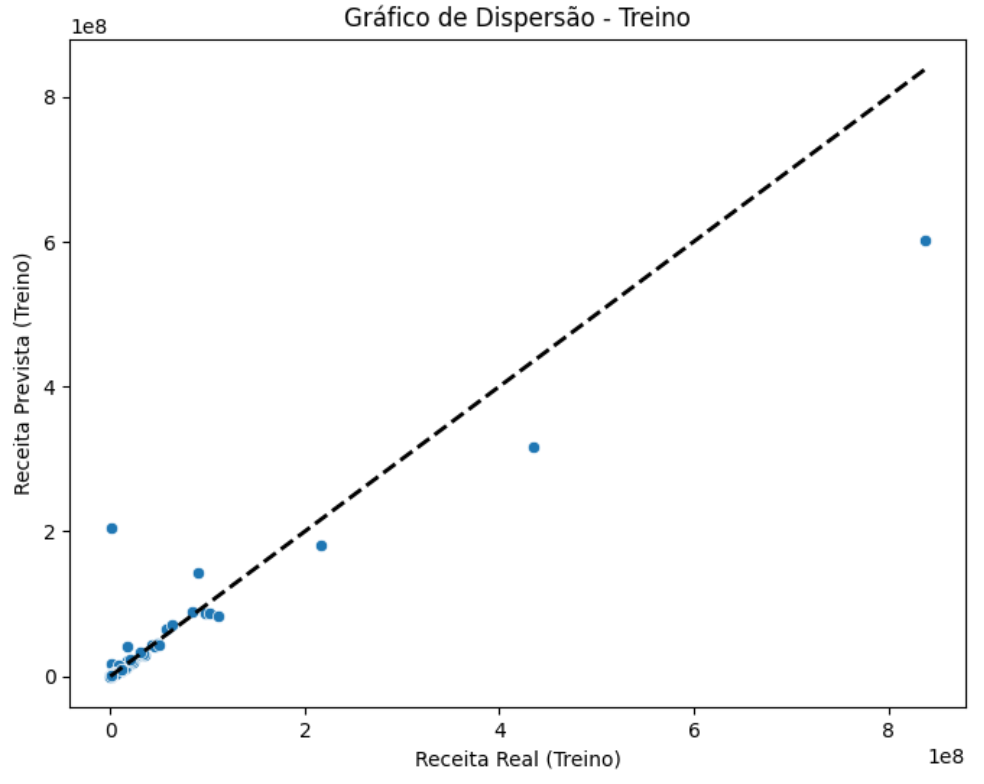
\includegraphics[width=0.5\linewidth]{graficoDispersaoTreino}
    \caption{Gráfico de Dispersão - Treino}
    \label{fig:enter-label}
\end{figure}

\begin{figure}
    \centering
    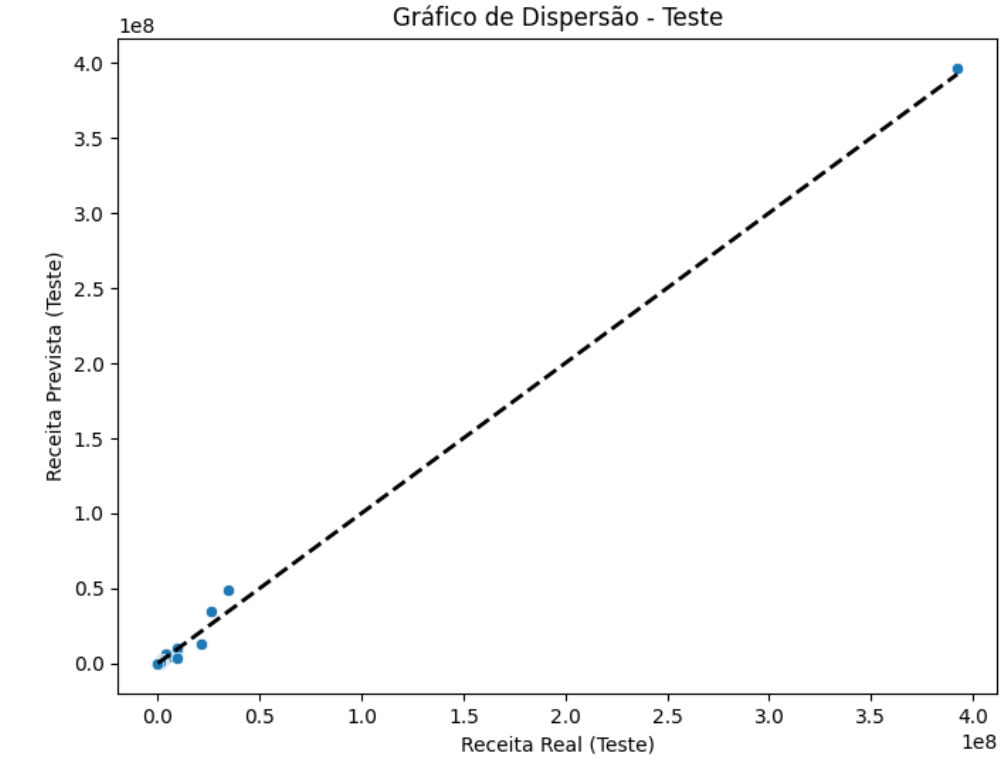
\includegraphics[width=0.5\linewidth]{graficoDispersaoTeste.png}
    \caption{Gráfico de Dispersão - Teste}
    \label{fig:enter-label}
\end{figure}


\section{Conclusão}

Este projeto demonstrou a aplicação de técnicas de aprendizado de máquina para prever a receita de jogos na Steam.  O modelo Random Forest obteve um alto R-squared no conjunto de treinamento, mas o RMSE e a análise dos gráficos de dispersão sugerem a possibilidade de overfitting.  Futuros trabalhos podem explorar técnicas para mitigar o overfitting, como regularização, aumento do conjunto de dados ou a utilização de modelos mais robustos à generalização.  A exploração de outras variáveis e a engenharia de novas features também podem contribuir para a melhoria do desempenho preditivo.

\section{Link Youtube}
https://www.youtube.com/watch?v=5xEPwh5dej0

\section{Bibliografia}

O dataset foi obtido em \cite{topcu2024top1500}.
Os slides de "Preparação e Pré-processamento dos dados" utilizados como base de 
estudo foram ministrados pelo Prof. Dr. Ivan Carlos Alcântara de Oliveira, sendo 
disponibilizados nas seguintes partes: 
\cite{professor_slides_2024parte1}, \cite{professor_slides_2024parte2} e 
\cite{professor_slides_2024parte3}.

\bibliographystyle{sbc}
\bibliography{sbc-template}

\end{document}
